\subsection{Scaling: Balancing Single- and Pair-Track Widths}
\label{sec:recipe-model-scaling}

\textbf{Explored designs.}
We study how the single-track width $d_s$ and pair-track width $d_p$ affect
performance when scaled independently or together. All other settings, including
depth, Pairmixer placement, conditioning, validation split, and sampler, are held
fixed. We report both the single-sample solve rate $\mathrm{Sol}_S$ and the
30-sample crystal-level solve rate $\mathrm{Sol}_C$, capturing per-sample success
and coverage across targets, respectively.

Starting from the base configuration W0 with $(d_s,d_p)=(512,128)$, we consider:
\begin{itemize}
    \item Pair scaling (W1, W2): increase $d_p$ to $192$ and $256$,
    respectively, while keeping $d_s=512$.
    \item Single scaling (W3, W5): increase $d_s$ to $768$ and $1024$,
    respectively, while keeping $d_p=128$.
    \item Balanced scaling (W4): increase both widths to
    $(d_s,d_p)=(768,192)$, preserving $d_s/d_p=4$.
\end{itemize}

\textbf{Scaling either width alone is insufficient.}
The epoch sweeps reveal distinct limitations of the two isolated scaling paths.
Increasing only the single width improves $\mathrm{Sol}_S$ but eventually reduces
$\mathrm{Sol}_C$, suggesting that the added capacity makes successes more
repeatable on already-solvable targets rather than expanding coverage. Increasing
only the pair width, in contrast, yields no consistent improvement in either
metric. Thus, neither isolated scaling path provides a uniformly better trade-off
across sampling budgets
(\Cref{fig:width-scaling-tradeoff}; \Cref{tab:width_scaling_ablation}).

\textbf{Balanced scaling reaches the sampling-budget Pareto frontier.}
Jointly scaling both widths allows W4 to maintain single-sample success while
recovering crystal-level coverage, yielding a better trade-off than scaling either
width alone. Adding weight decay of $10^{-2}$ shifts W4 toward greater coverage,
trading some success at $k{=}1$ for improved coverage at $k{=}30$. We prioritize
coverage because CSP workflows generate multiple candidates for subsequent ranking;
a structure absent from the candidate set cannot be recovered downstream
\citep{hunnisett2024seventhranking,hunnisett2024seventhgeneration}.
We therefore retain W0 as \model{}-M and select W4 with weight decay
$10^{-2}$ as \model{}-L (\Cref{fig:width-scaling-tradeoff}).

\begin{figure}[t]
  \centering
  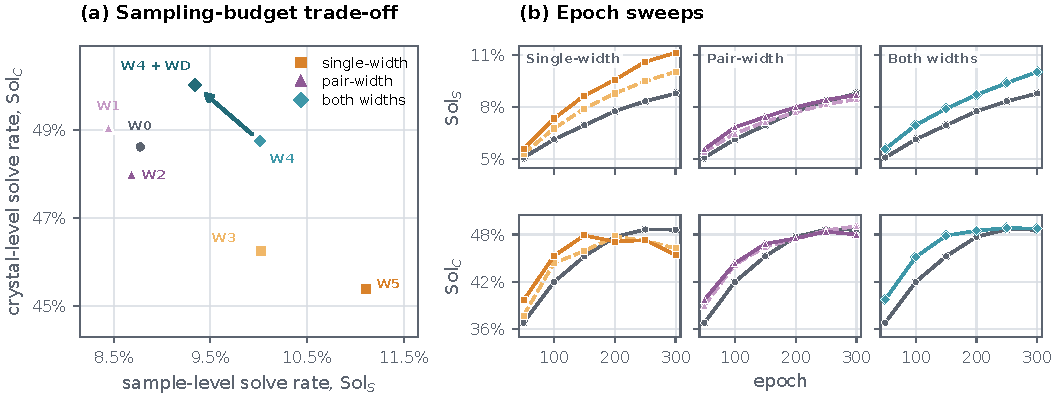
\includegraphics[width=\textwidth]{figures/generated/fig_width_scaling_tradeoff.pdf}
  \caption{\textbf{Balanced width scaling reaches the sampling-budget Pareto
    frontier.} \textbf{(a)} Single-sample solve rate
    $\mathrm{Sol}_S$ ($k{=}1$) versus crystal-level solve rate
    $\mathrm{Sol}_C$ at $k{=}30$ at epoch 300. Marker shape and color indicate the
    width-scaling family. Scaling either the single or pair width alone does not
    consistently improve the trade-off between per-sample success and target
    coverage, whereas jointly scaling both widths reaches the Pareto frontier.
    Adding weight decay of $10^{-2}$ further shifts the balanced model toward
    higher $k{=}30$ coverage. W0 is selected as \model{}-M, and W4 with weight
    decay (W4 + WD) as \model{}-L. \textbf{(b)} Epoch sweeps for single-width
    scaling (W0, W3, W5), pair-width scaling (W0, W1, W2), and balanced scaling
    (W0, W4). Top and bottom rows report $\mathrm{Sol}_S$ and $\mathrm{Sol}_C$,
    respectively. All metrics use the shared validation protocol with 30
    candidates per target and 200-step EDM--Heun sampling.}
  \label{fig:width-scaling-tradeoff}
\end{figure}

\begin{table}[!t]
\centering
\caption{\textbf{Width-scaling ablation.}
All rows keep depth, Pairmixer placement, conditioning, validation split, and
sampler fixed while varying the single width $d_s$ and pair width $d_p$.
$\mathrm{Sol}_S$ and $\mathrm{Sol}_C$ are evaluated at epoch 300 with 30
candidates per target and 200-step EDM--Heun sampling (400 NFE). GFLOPs denote
analytical denoiser-forward costs at $N{=}300$. Teal rows mark the selected width
configurations: W0 defines \model{}-M, while W4 defines the width of \model{}-L
before applying weight decay as selected in \Cref{fig:width-scaling-tradeoff}.}
\label{tab:width_scaling_ablation}
\small
\begin{tabular}{@{}lccccccc@{}}
\toprule
ID & $d_s$ & $d_p$ & Heads & Params (M) & GFLOPs &
$\mathrm{Sol}_S \uparrow$ & $\mathrm{Sol}_C \uparrow$ \\
\midrule
\rowcolor{mfTealFill}
W0 & 512 & 128 & 8 & 87.56 & 379.6 & 0.088 & 0.486 \\
W1 & 512 & 192 & 8 & 89.65 & 762.6 & 0.084 & 0.490 \\
W2 & 512 & 256 & 8 & 92.54 & 1287.2 & 0.087 & 0.480 \\
W3 & 768 & 128 & 12 & 184.79 & 421.0 & 0.100 & 0.462 \\
\rowcolor{mfTealFill}
W4 & 768 & 192 & 12 & 186.91 & 804.7 & 0.100 & 0.487 \\
W5 & 1024 & 128 & 16 & 330.79 & 483.8 & 0.111 & 0.454 \\
\bottomrule
\end{tabular}
\end{table}

